%%=========================================
\chapter{Results and Discussion}\label{ch:results-and-discussion}
In this chapter, experimental results are presented, analysed, and discussed. In total, one (111)B substrate from vendor A (substrate A), two (111)B substrates from vendor B (substrate B and B2), and one (211)B substrate from vendor A (substrate C) were investigated using bright and dark field microscopy, \ac{sem}, \ac{eds}, \ac{afm}, near-\ac{ir} transmission microscopy, and \ac{ftir}. Except for substrate B2, which was only investigated after surface pre-growth preparation, the substrates were investigated both as-received and after surface pre-growth preparation.%\todo{, and after \ac{mct} growth.}
%%=========================================

\section{Surface Analysis of As-Received Substrate A}\label{sec:subAa}
% Substrate A
In previous work \citep{lauten2017characterisation}, the state-of-the-art as-received (111)B-oriented substrate A was characterised for polishing damage, defects, and residual particles using optical microscopy, \ac{sem} with \ac{eds}, and \ac{xps}. The results are reiterated in this section to better present the full scope of the study. In addition to the previously used methods, \ac{afm}, near-\ac{ir} transmission microscopy, and \ac{ftir} were used to study the as-received substrate.

Fig.~\ref{fig:subAa_om_df} shows dark field images from the surface of substrate A at the corner, edge, and centre of the substrate. The highly polished (111)B surface is smooth and only a few particles or morphological defects can be seen. By counting the number of spots in the dark field image, the particle and morphological defect density was estimated to be \SI{4e2}{\centi\metre^{-2}} at the centre and \SI{1e3}{\centi\metre^{-2}} at the edges and corners of the surface of substrate A. Here the particle and morphological defect density refers to the sum of all light scattering objects with sizes \SI{>0.5}{\micro\metre} since any particles or morphological defects that have sizes \SI{<0.5}{\micro\metre} are not seen in the dark field images. Therefore, the true morphological defect density was higher than the one estimated from the dark field images.
% --- Measured with tolerance of 7 using ImageJ.
%       Centre: 17 partikler på 2048x1536
%       Corner: 30 partikler på 1732x1327

\begin{figure}[htbp]
    \centering
    \mySubfigure[Corner.]{0.48\textwidth}{LM_DF_BZ1503ID71A_M005_corner_with_skraa.jpg}
    %\quad
    \mySubfigure[Edge.]{0.48\textwidth}{LM_DF_BZ1503ID71A_M005_edge.jpg}
    \par\bigskip
    \mySubfigure[Centre.]{\linewidth}{LM_DF_BZ1503ID71A_M005_centre.jpg}
    \caption[Dark field images of substrate A.]{Dark field images of substrate A captured through the optical microscope Leica DM RXA2 at a magnification of 5$\times$.}
    \label{fig:subAa_om_df}
\end{figure}

The \ac{sem} image in Fig.~\ref{fig:EDX_BZ1503A_a_m001}, taken at a magnification of 100, shows that the surface of substrate A is smooth with few particles and defects. Some bright spots, that correspond to an irregularity on the surface, can be seen in the image. These features become easier to detect at a magnification of 3500$\times$, see Fig.~\ref{fig:substrateA_a2_m005}, where eleven bright spots and two straight lines can be seen. These features need to be studied at even higher magnifications to be able to identify what they are.
\begin{figure}[htbp]
    \centering
    \mySubfigure[SEM image at a magnification of 100$\times$.]{0.48\linewidth}{EDX_BZ1503A_a_m001.jpg}[fig:EDX_BZ1503A_a_m001]
    \mySubfigure[SEM image at a magnification of 3500$\times$.]{0.48\linewidth}{substrateA_a2_m005.jpg}[fig:substrateA_a2_m005]
    \caption[SEM images of substrate A.]{Scanning electron microscopy (SEM) images of surface of substrate A.}
    \label{fig:subA_overview}
\end{figure}
% A particle and morphological defect density of features \SI{>0.5}{\micro\metre} of \SI{4e2}{\centi\metre^{-2}} at the centre and \SI{1e3}{\centi\metre^{-2}} at the edges of the substrate was observed. Substrate A had polishing scratches that were between 10 and \SI{20}{\nano\metre} wide. In addition, pieces of residual polishing grit was found on the surface. An \ac{eds} spectrum of an agglomeration of multiple particles revealed that they were composed of alumina (\ce{Al2O3}) and silica (\ce{SiO2}) polishing grit. In addition, larger particles with size of \SI{\sim 10}{\micro\metre} on the substrate surface were observed. \Ac{eds} revealed that these particles mainly consisted of titanium.

%%=========================================
\subsection{Particles}
Four different types of particles were observed on the surface of substrate A, see Fig.~\ref{fig:subAa_sem_w_eds}. They will be described and identified in the following. It was difficult to focus on the surface due to the uniformity of the substrate. Hence, there are no density measurements for the as-received substrate A.

\begin{figure}
    \centering
    \begin{subfigure}[t]{\textwidth}
          \begin{minipage}[t]{0.49\linewidth}
            \centering
            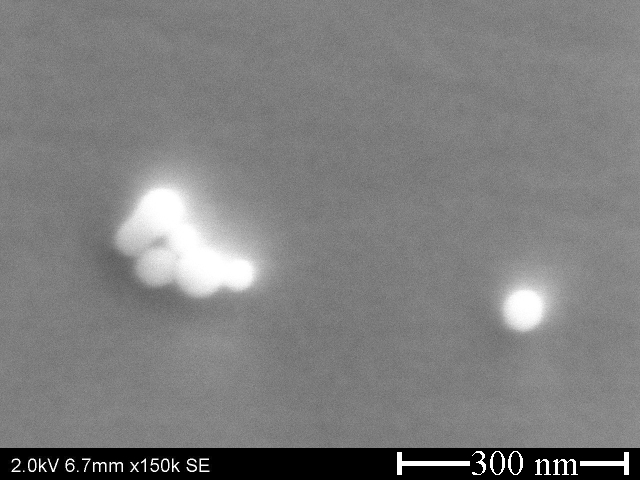
\includegraphics[width=\linewidth]{substrateA_a2_m006.jpg}
          \end{minipage}
          \hfill
          \begin{minipage}[t]{0.49\linewidth}
            \centering
            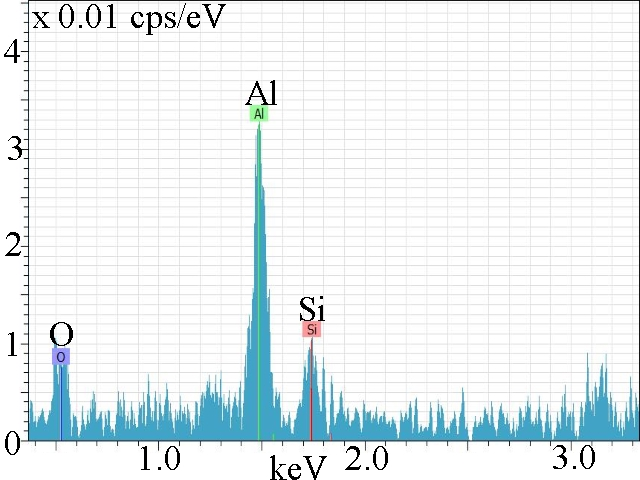
\includegraphics[width=\linewidth]{subA_eds_alumina02.jpg}
          \end{minipage}
        \caption{The \ac{sem} image show an agglomeration of polishing grit particles and one single polishing grit particle with a diameter of \SI{50}{\nano\metre}. The corresponding \ac{eds} spectrum reveals that the agglomeration consist of \ce{Al2O3}, also known as alumina.}\label{fig:subAa_polishing-grit}
    \end{subfigure}
    \par\bigskip
    \begin{subfigure}[t]{\textwidth}
          \begin{minipage}[t]{0.49\linewidth}
            \centering
            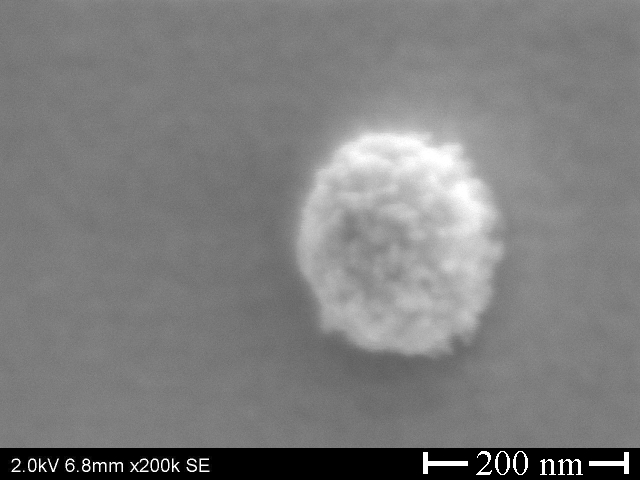
\includegraphics[width=\linewidth]{substrateA_a1_m016.jpg}
          \end{minipage}
          \hfill
          \begin{minipage}[t]{0.49\linewidth}
            \centering
            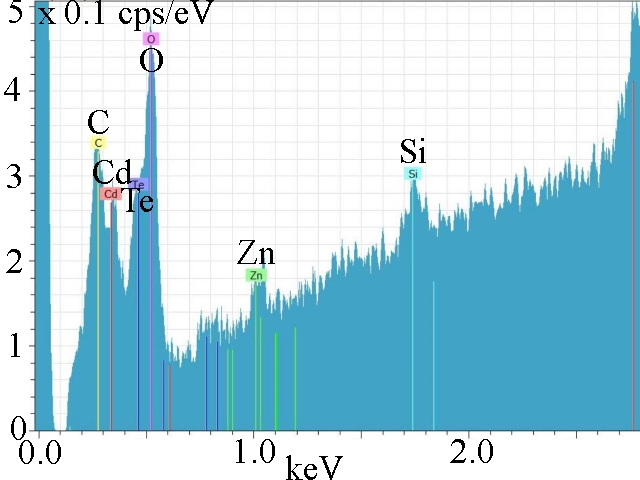
\includegraphics[width=\linewidth]{eds_subA_SiO2.jpg}
          \end{minipage}
        \caption{A particle with a diameter of \SI{200}{\nano\metre}. The \ac{eds} spectrum of the particle reveals that the particle consists of \ce{Si}, \ce{C} and \ce{O}.}\label{fig:subAa_large-grit}
    \end{subfigure}
    \par\bigskip
    \begin{subfigure}[t]{\textwidth}
          \begin{minipage}[t]{0.49\linewidth}
            \centering
            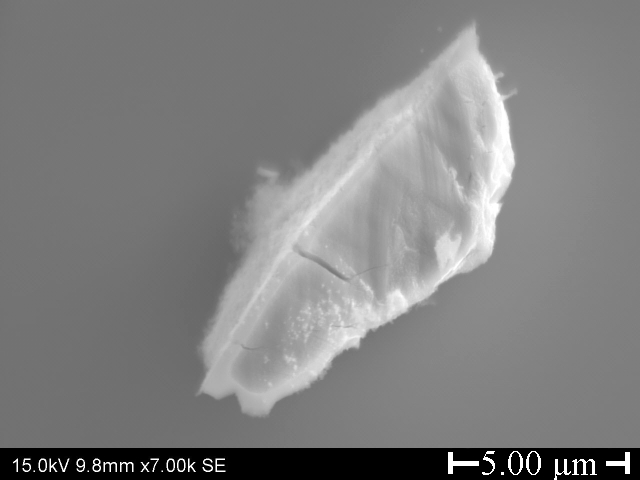
\includegraphics[width=\linewidth]{substrateA_a2_m011.jpg}
          \end{minipage}
          \hfill
          \begin{minipage}[t]{0.49\linewidth}
            \centering
            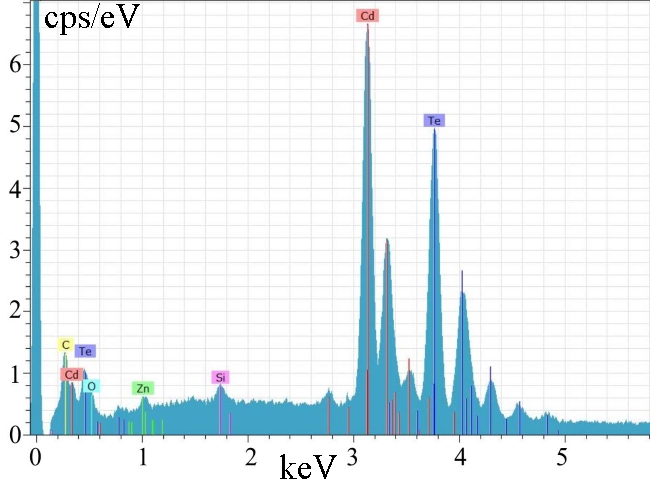
\includegraphics[width=\linewidth]{eds_subA_CZT.jpg}
          \end{minipage}
        \caption{A \SI{12}{\micro\metre} long particle having the same composition as the underlying substrate.}\label{fig:subAa_czt-particle}
    \end{subfigure}
    \caption[\Ac{sem} images and \ac{eds} spectra of particles found on as-received substrate A.]{High resolution \acf{sem} images of particles found on the as-received substrate A and the corresponding \acf{eds} spectra of the particles.}\label{fig:subAa_sem_w_eds}
\end{figure}

\begin{figure}[htbp]
\ContinuedFloat
    \centering
    \begin{subfigure}[t]{\textwidth}
          \begin{minipage}[t]{0.49\linewidth}
            \centering
            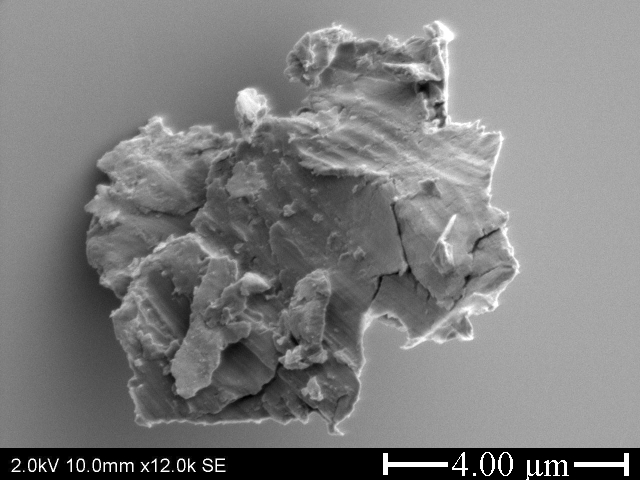
\includegraphics[width=\linewidth]{titan_sem.jpg}
          \end{minipage}
          \hfill
          \begin{minipage}[t]{0.49\linewidth}
            \centering
            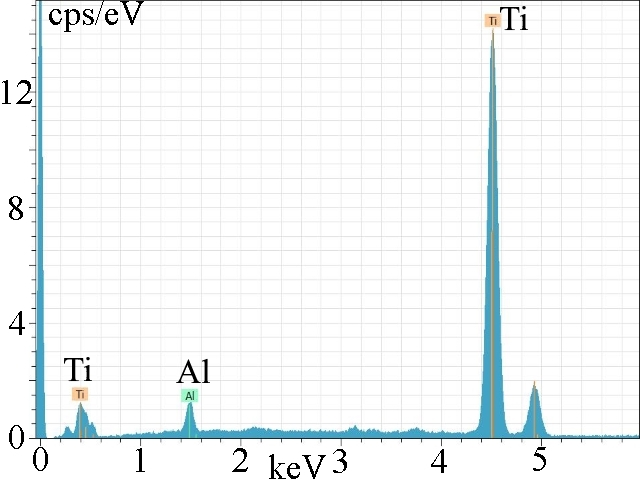
\includegraphics[width=\linewidth]{titan_eds.jpg}
          \end{minipage}
        \caption{An \SI{8}{\micro\metre} long particle consisting of mainly titanium.}\label{fig:subAa_titanium-particle}
    \end{subfigure}
    \captionsetup{list=no}
    \caption{\emph{(continued)}}
\end{figure}

%\subsubsection{Type A.I}
Small particles of size \SI{50}{\nano\metre} were spread scarcely out over the surface of substrate A. It seems like they are easier to observe near the edges of the substrate and therefore have a higher density towards the edges than in the centre, but this could also be due to the difficulties of focusing the \ac{sem} beam on the flat surface. Fig.~\ref{fig:subAa_polishing-grit} shows one large piece and one small piece of this type of particle along with the corresponding \ac{eds} spectrum of the large piece. The large piece is an agglomeration of the smaller ones. \ac{eds} reveals that the larger piece consists of \ce{Al}, \ce{Si} and \ce{O}. The particles are most likely residual \ce{Al2O3} and \ce{SiO2} polishing grit which are commonly used in polishing slurries \citep{benson2015as-received}.

\begin{comment}
\begin{figure}[htbp]
    \centering
    \subfigure[SEM image at a magnification of 150000$\times$.]{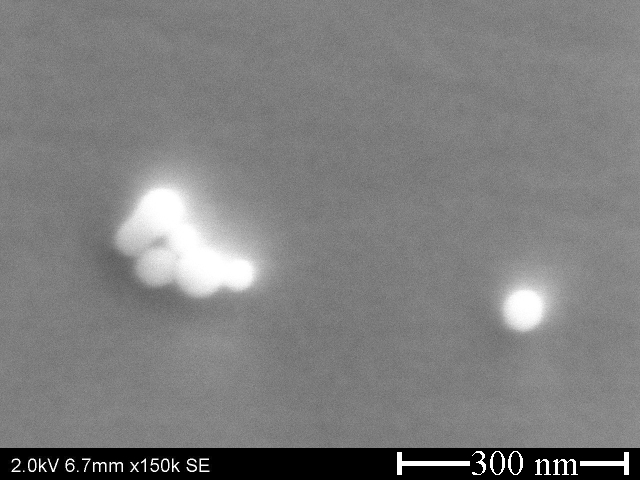
\includegraphics[width=0.48\linewidth]{substrateA_a2_m006.jpg}\label{fig:substrateA_a2_m006}}
    \subfigure[EDS.]{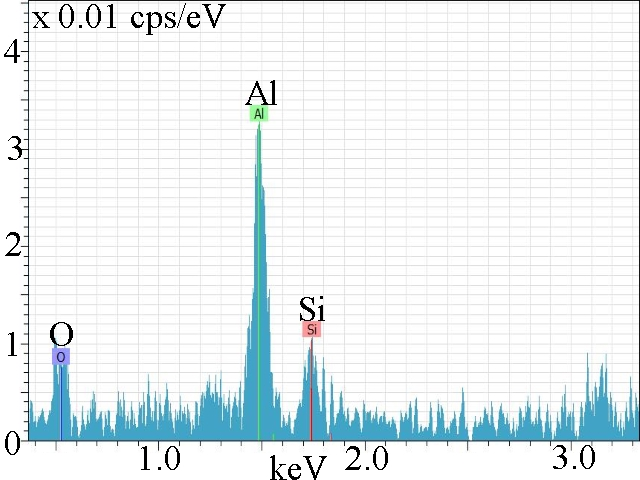
\includegraphics[width=0.48\linewidth]{subA_eds_alumina02.jpg}\label{fig:subA_eds_alumina02}}
    \caption[ SEM image and EDS spectrum of a particle on substrate A.]{High resolution scanning electron microscopy (SEM) image of one large and small piece of particles on substrate A and the corresponding \acf{eds} spectrum of the large piece.}
    \label{fig:subA_alumina}
\end{figure}
\end{comment}

%\subsubsection{Type A.II}
A particle with a diameter of \SI{200}{\nano\metre} is shown in Fig.~\ref{fig:subAa_large-grit} with the corresponding \ac{eds} spectrum. This particle is considerably larger and has a rougher surface than the more frequently observed \SI{50}{\nano\metre} particles that were found to be residual polishing grit. The \ac{eds} spectrum of the particle reveals that the particle consists of \ce{Si}, \ce{C} and \ce{O}, which indicates that also this particle could be residual \ce{SIO2} polishing grit, \ce{SiC} polishing grit, or an agglomeration of both.

\begin{comment}
\begin{figure}[htbp]
    \centering
    \subfigure[SEM image at a magnification of 200000$\times$.]{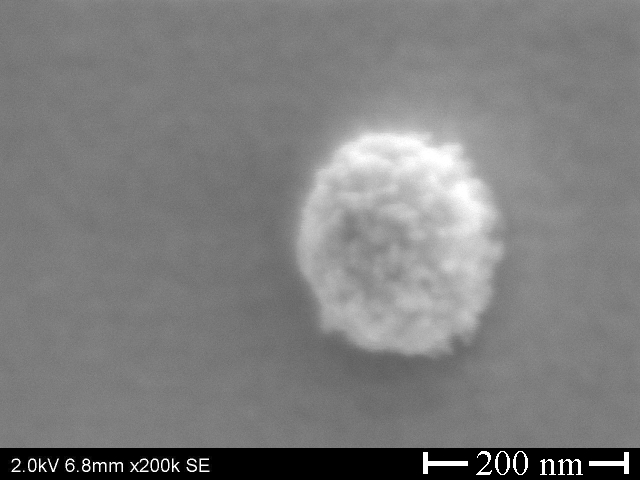
\includegraphics[width=0.48\linewidth]{substrateA_a1_m016.jpg}\label{fig:substrateA_a1_m016}}
    \quad
    \subfigure[EDS.]{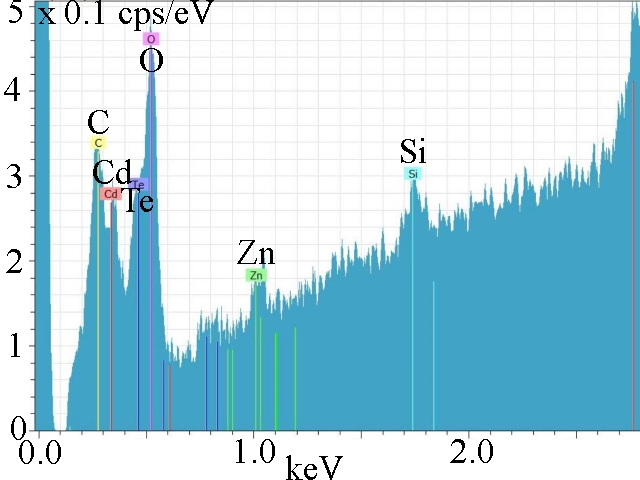
\includegraphics[width=0.48\linewidth]{eds_subA_SiO2.jpg}\label{fig:subA_200nm_eds}}
    \caption[]{High resolution scanning electron microscopy (SEM) image and the corresponding \acf{eds} spectrum of a particle on substrate A at a magnification of 200000$\times$).}
    \label{fig:subA_partII}
\end{figure}
\end{comment}

Particles with size \SI{>5}{\micro\metre} are observed mainly near the edges of substrate A. Fig.~\ref{fig:subAa_czt-particle} shows a particle that is \SI{13}{\micro\metre} long and \SI{5}{\micro\metre} wide. A comparison between the corresponding \ac{eds} spectrum of the particle and the substrate surface spectrum reveals that the particle consists of the same material as the substrate and that it could be debris from the cutting and polishing of the substrate at the vendor.

\begin{comment}
\begin{figure}[htbp]
    \centering
    \subfigure[SEM image at a magnification of 7000$\times$.]{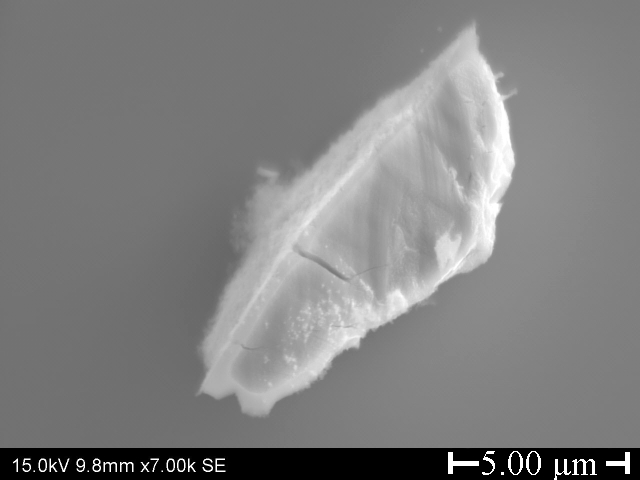
\includegraphics[width=0.48\linewidth]{substrateA_a2_m011.jpg}\label{fig:substrateA_a2_m011}}
    \quad
    \subfigure[EDS.]{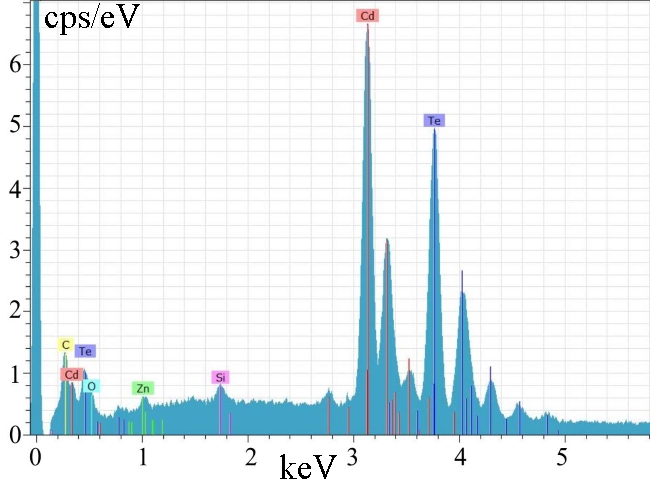
\includegraphics[width=0.48\linewidth]{eds_subA_CZT.jpg}\label{fig:eds_subA_CZT}}
    \caption[]{Scanning electron microscopy (SEM) image and the corresponding \acf{eds} spectrum of a particle on substrate A at a magnification of 7000$\times$).}
    \label{fig:subA_czt}
\end{figure}
\end{comment}

Fig.~\ref{fig:subAa_titanium-particle} shows a particle that is \SI{8}{\micro\metre} long and \SI{4}{\micro\metre} wide. The corresponding \ac{eds} spectrum of the particle reveals that the particle consists of titanium. The particle has sharp edges and are therefore not used as polishing grit since the edges had been rounded in that case. It could be a debris coming from vendor A, but most likely it comes from the substrate holder for the \ac{xps} measurements. The holder was new, made out of titanium in the machine shop, and it seems some particles were created during mounting.

\begin{comment}
\begin{figure}[htbp]
    \centering
    \subfigure[SEM image at a magnification of 12000$\times$.]{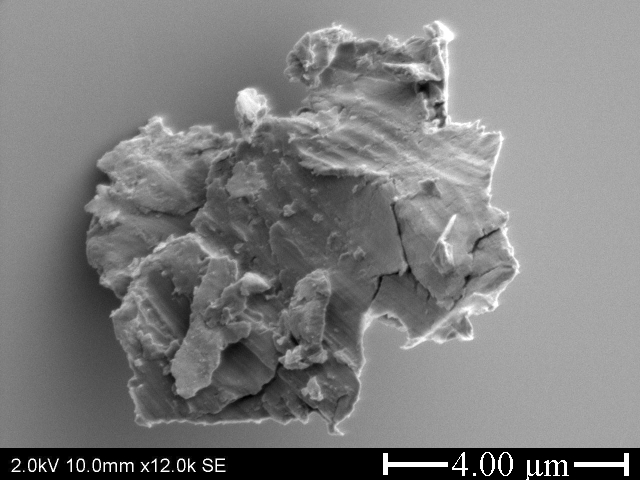
\includegraphics[width=0.48\linewidth]{titan_sem.jpg}\label{fig:titan_sem}}
    \quad
    \subfigure[EDS.]{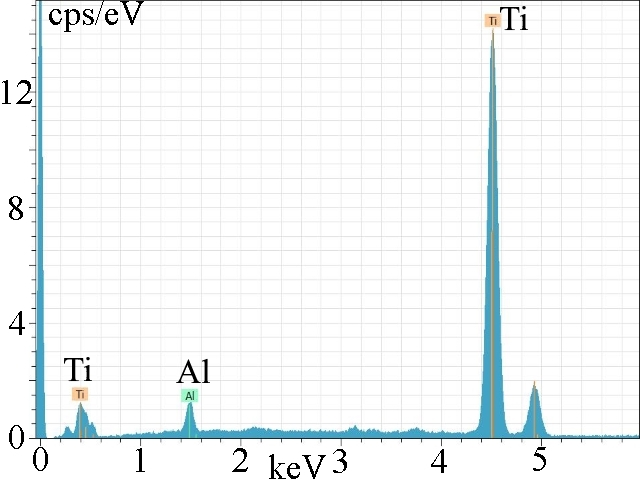
\includegraphics[width=0.48\linewidth]{titan_eds.jpg}\label{fig:titan_eds}}
    \caption[]{Scanning electron microscopy (SEM) image and the corresponding \acf{eds} spectrum of a particle on substrate A at a magnification of 12000$\times$).}
    \label{fig:subA_Ti}
\end{figure}
\end{comment}

%%=========================================

\Ac{sem} and \ac{eds} measurements of particles from the \ac{xps} holder, collected with an adhesive carbon tab, confirms that the same type of titanium particles were found on the \ac{xps} holder. This fact, shows how important it is to clean the equipment carefully before use. %see Fig.~\ref{fig:subAa_titanium}

\begin{comment}
\begin{figure}[htbp]
    \centering
      \begin{minipage}[t]{0.49\linewidth}
        \centering
        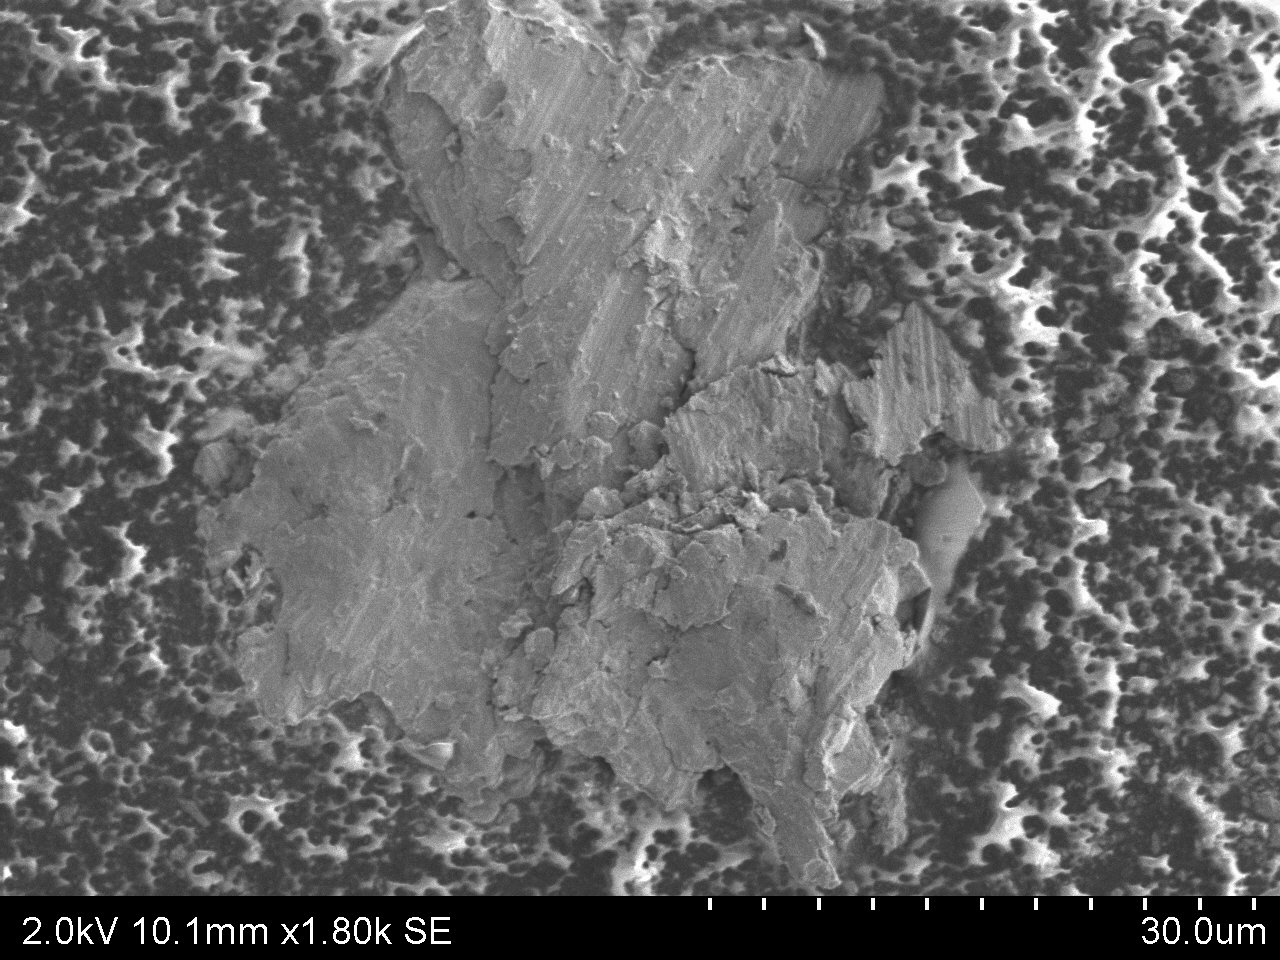
\includegraphics[width=\linewidth]{subAa_sem-holder_b_m001.jpg}
      \end{minipage}
      %\hfill
      \begin{minipage}[t]{0.49\linewidth}
        \centering
        
\includegraphics[width=\linewidth]{unknown.png}
      \end{minipage}
    \caption[\Ac{sem} image and corresponding \ac{eds} spectrum of titanium particle.]{A \ac{sem} image and the corresponding \ac{eds} spectrum of a titanium particle found on the holder used to transport substrates into the \ac{xps} chamber. The particles is \SI{8}{\micro\metre} long and consisting mainly of titanium. A carbon tab can be seen under the particle.}
    \label{fig:subAa_titanium}%[fig:subAa_eds_titanium]%\label{fig:subAa_sem_titanium}}
\end{figure}
\end{comment}

%%=========================================

\subsection{Surface Scratches and Roughness}
The as-received surface of substrate A was carefully polished and the typical surface scratches are between \SI{10} and {}\SI{20}{\nano\metre} wide, as seen in Fig.~\ref{fig:subAa_scratches}. However, some wider surface scratches with a width of \SI{0.1}{\micro\metre} was observed as well. The surface scratches most likely have shallow depth since they cannot be seen in the dark field images of substrate A.

\begin{figure}[htbp]
    \centering
    %\subfigure[High resolution SEM at SEM image at a magnification of 80000$\times$.]{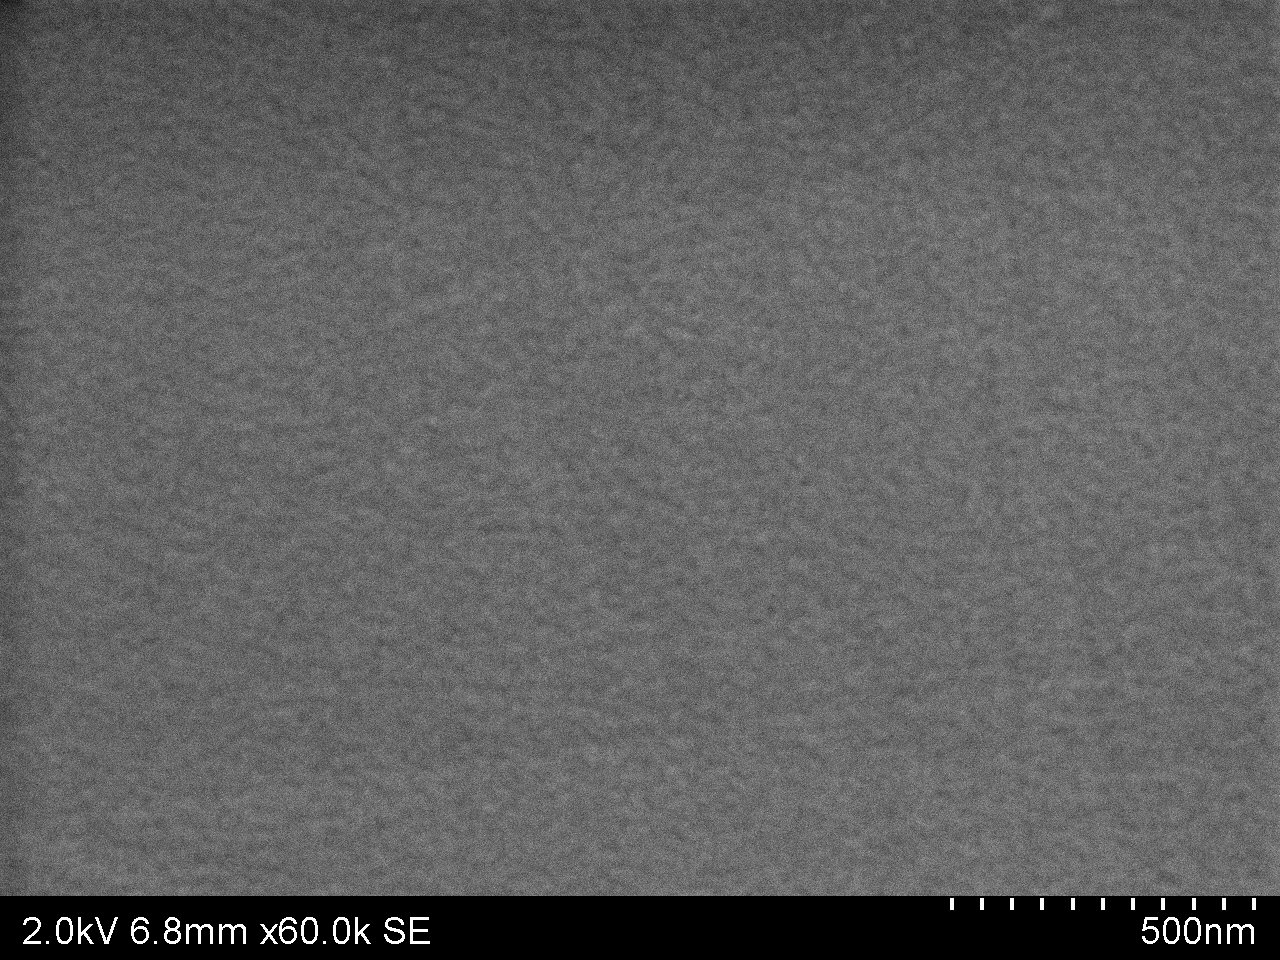
\includegraphics[width=0.48\linewidth]{substrateA_a2_m003.jpg}\label{fig:substrateA_a2_m003}}
    %\quad
    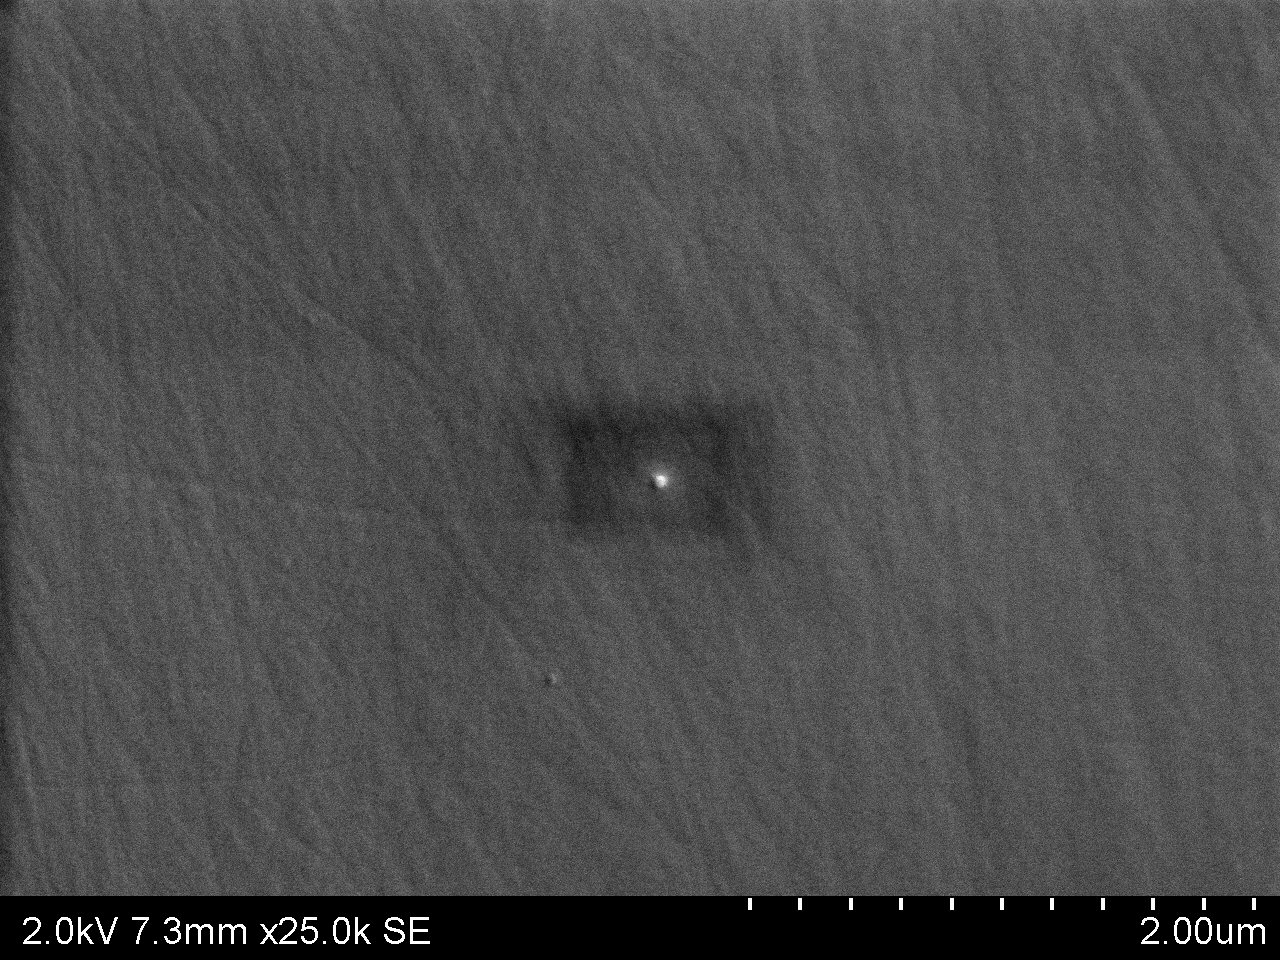
\includegraphics[width=0.75\linewidth]{substrateA_a1_m011.jpg}
    \caption[\Ac{sem} image of surface scratches on substrate A.]{High resolution \acf{sem} image of the surface of substrate A at a magnification of 25000$\times$. The dark square is carbon deposited on the surface while focusing the beam at a higher magnification.}\label{fig:subAa_scratches}
    \label{fig:SEM_A_surface}
\end{figure}

%%=========================================
%\section{AFM Study of As-Received Substrate A}
The as-received substrate A was characterised for surface topography by \ac{afm}. Fig.~\ref{fig:afm_subA} show \ac{afm} images of the surface. The \ac{rms} roughness of substrate A is \SI{\sim0.3}{\nano\metre} at both the centre and around the edges. This indicates the absence of large scratches. The largest polishing scratches on substrate A are \SI{0.2}{\micro\metre} wide and \SI{1}{\nano\metre} in depth.


\begin{figure}[htbp] % left lower right upper
    \centering
    \begin{subfigure}[t]{0.5\linewidth}
        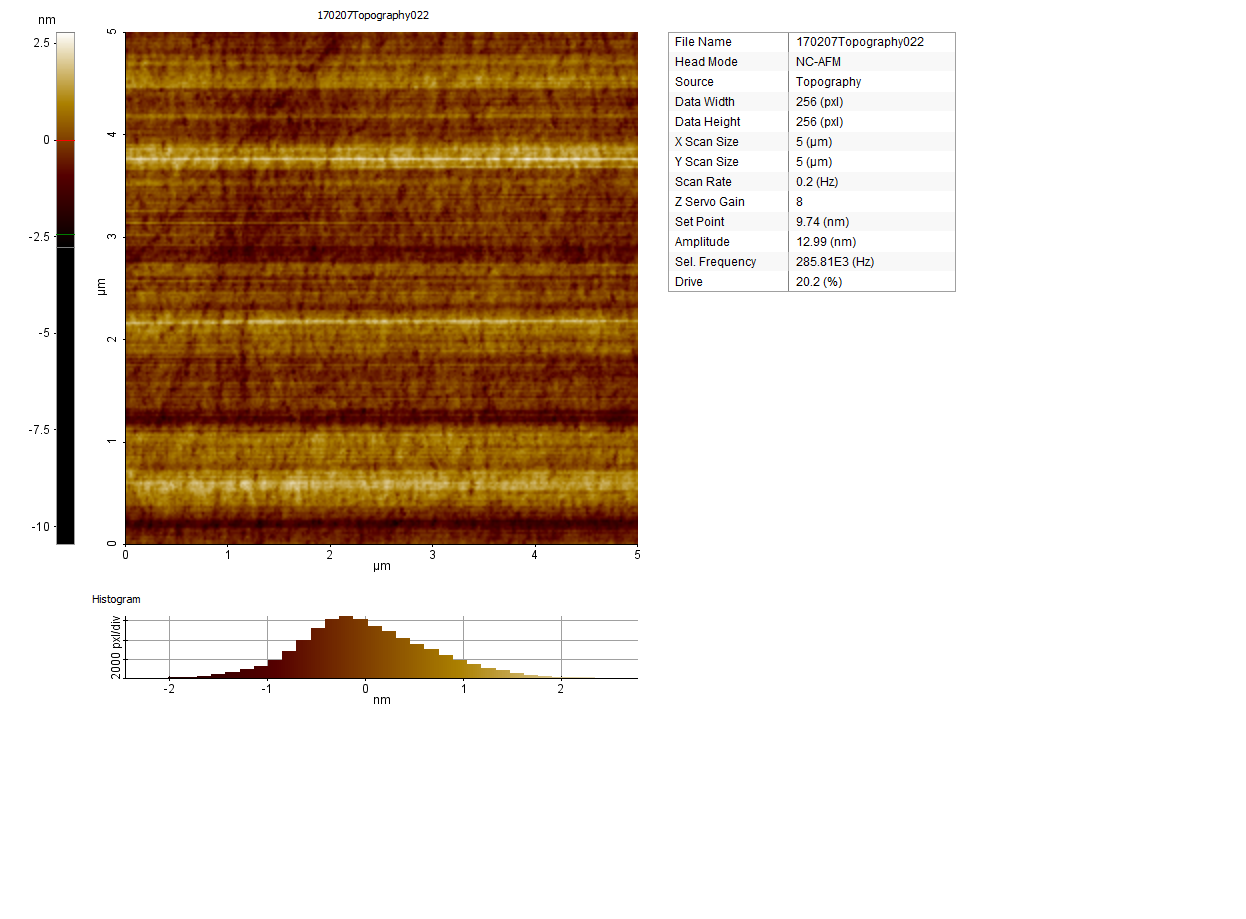
\includegraphics[width=\linewidth,trim={0cm 12cm 21cm 0cm},clip]{170207Topography022.png}
        \caption{Near centre, \ac{rms} roughness \SI{0.31}{\nano\metre}.}%
    \end{subfigure}
    \par\bigskip
    \begin{subfigure}[t]{0.5\linewidth}
        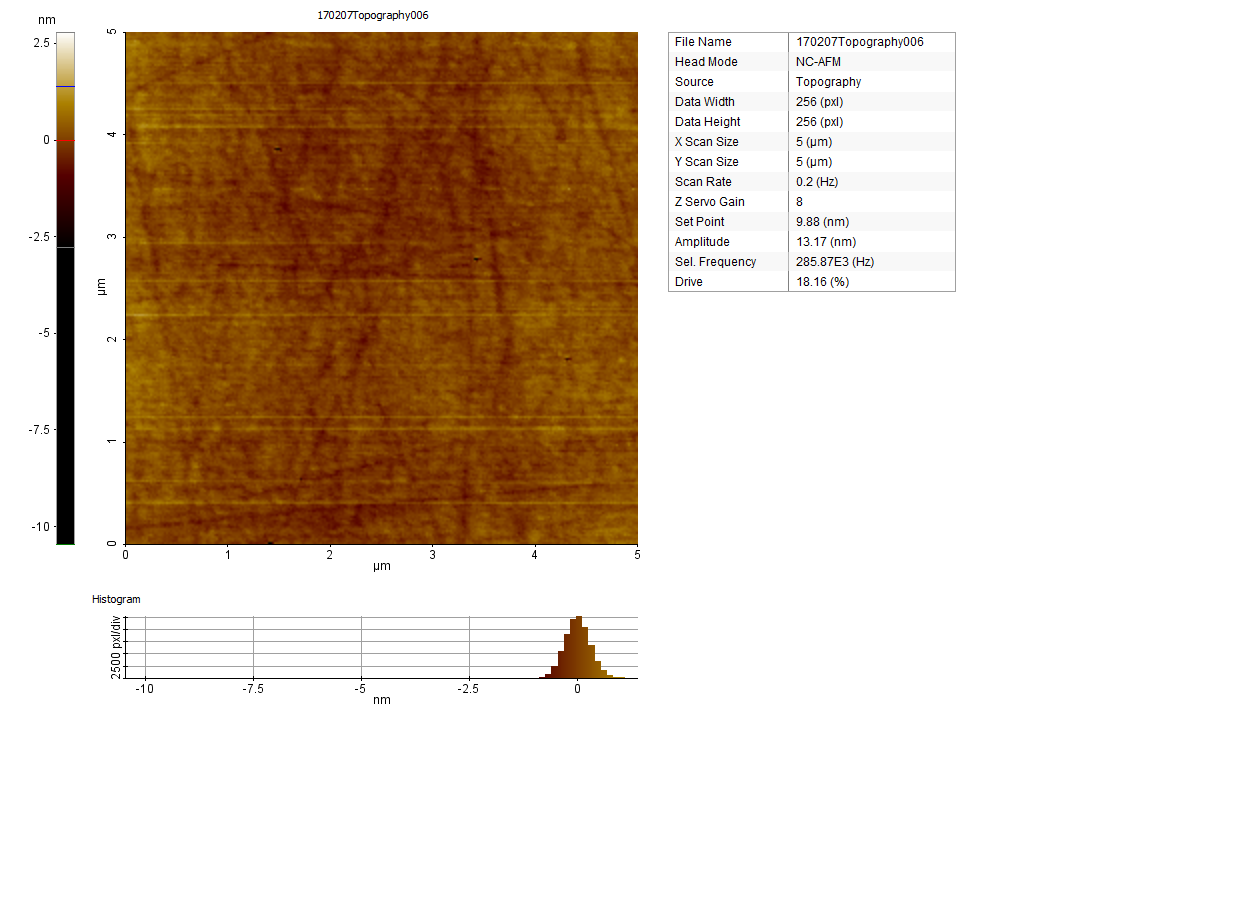
\includegraphics[width=\linewidth,trim={0cm 12cm 21cm 0cm},clip]{170207Topography006.png}
        \caption{Near upper edge, \ac{rms} roughness \SI{0.30}{\nano\metre}.}%0,26
    \end{subfigure}
    \par\bigskip
    \begin{subfigure}[t]{0.5\linewidth}
        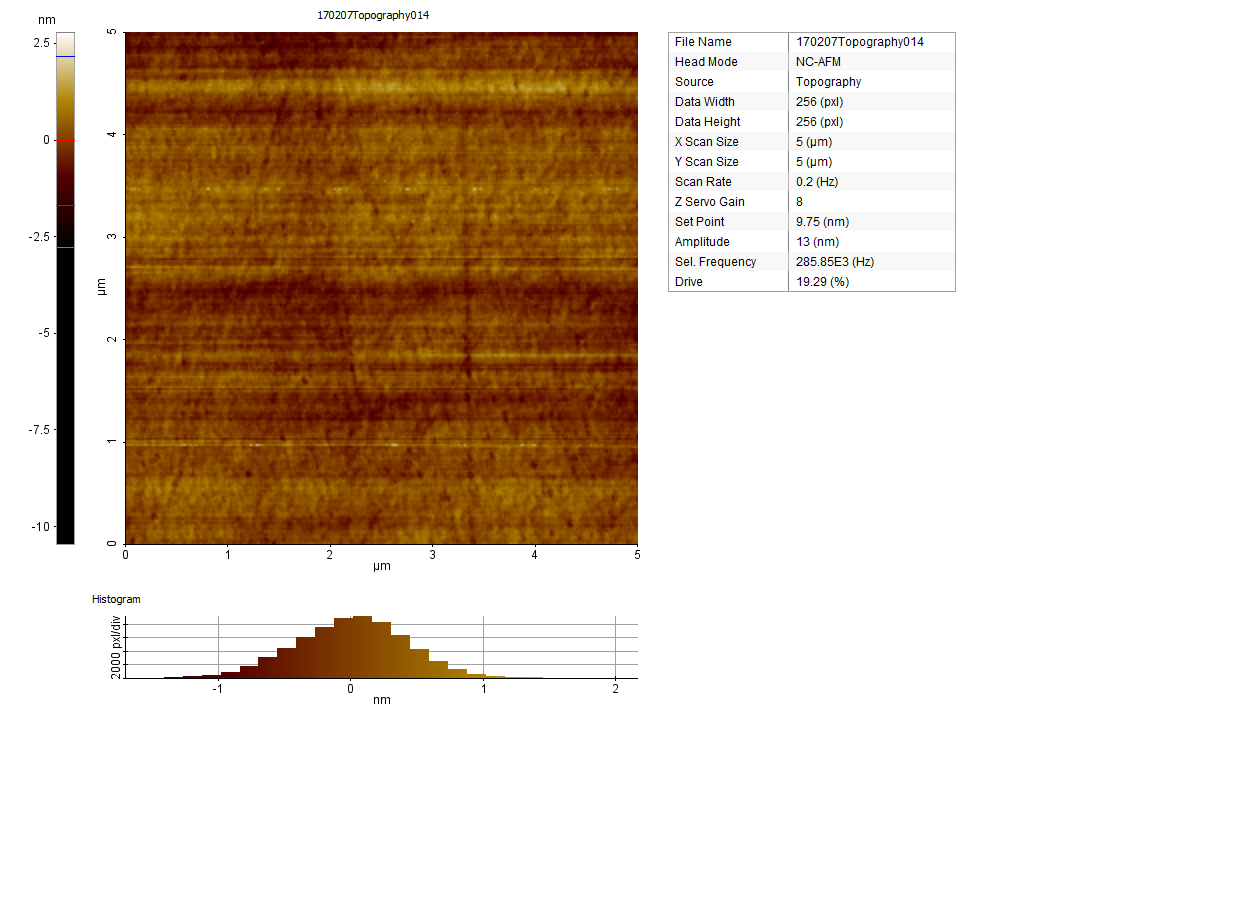
\includegraphics[width=\linewidth,trim={0cm 12cm 21cm 0cm},clip]{170207Topography014.png}
        \caption{Near upper left corner, \ac{rms} roughness \SI{0.41}{\nano\metre}.}%0,26
    \end{subfigure}
    \caption[\Ac{afm} of as-received substrate A.]{\Acf{afm} measurements of the as-received substrate A. Images of a $\SI{5}{\micro\metre}\times\SI{5}{\micro\metre}$ area are taken at the centre, edge, and corner of the substrate.}\label{fig:afm_subA}
\end{figure} % AFM, substrate A, as-received.



%%=========================================
%\section{Near-IR of As-Received Substrate A}

%%=========================================
\subsection{Impurity Analysis}

\Ac{xps} analysis was performed on the as-received substrate A to determine the composition of the outermost layers of the substrate (\SI{\sim 80}{\angstrom}). The centre of the $30\times\SI{30}{\milli\metre^2}$ \ce{CdZnTe} wafer was analysed using \ac{xps}. With the large beam size of \SI{1}{\centi\metre}, it should be possible to see traces of impurity elements over a large area, but not locate them to specific particles or small areas. Unfortunately, something was broken on the old analyser, resulting in low signal intensity and no detection of impurities or small concentrations of elements. The ever-present oxide and carbon overlayers further decreased any small signals. Therefore, the XPS only gave information about the following elements: \ce{Te}, \ce{Cd}, \ce{O}, and \ce{C}, see Fig.~\ref{fig:xps_spectra}. The reason for not performing \ac{xps} analysis on substrate B was that it would not be possible to detect the presence of impurities or small concentrations of elements with the \ac{xps} equipment at hand.

\begin{figure}[htbp]
    \centering
    \mySubfigure[\ce{Te} 3d spectrum with extra peak due to \ce{Te} oxide.]{0.44\linewidth}{xps_Te3d.png}[fig:xps_Te3d]
    \mySubfigure[\ce{Cd} 3d spectrum.]{0.48\linewidth}{xps_Cd3d.png}[fig:xps_Cd3d]
    \mySubfigure[\ce{O} 1s spectrum.]{0.48\linewidth}{xps_O1s.png}[fig:xps_O1s]
    \mySubfigure[\ce{C} 1s spectrum.]{0.48\linewidth}{xps_C1s.png}[fig:xps_C1s]
    \caption[\Ac{xps} spectra from substrate A.]{\Acf{xps} spectra from substrate A that displays the number of detected electrons (counts) as a function of their corresponding binding energy, $E_\mathrm{B}$ (\SI{}{\electronvolt}). The spectra were acquired using the \ce{Mg} anode.}
    \label{fig:xps_spectra}
\end{figure}
 
The atomic concentrations were calculated using Eq.~\eqref{eq:xps_concentration} with intensity peak areas and the following experimentally measured atomic sensitivity factors, determined earlier at \ac{ffi} \citep{hirsch1999x-ray}: \ce{Cd} 3d\textsubscript{5/2} (0.56), \ce{Te} 3d\textsubscript{5/2} (1.00), \ce{O} 1s (0.13), and \ce{C} 1s (0.05). Table~\ref{tab:xps_results} displays the results of the \ac{xps} analysis of substrate A. \ce{Cd_{0.96}Zn_{0.04}Te} should consist of \SI{48}{\atomic\percent} cadmium, \SI{2}{\atomic\percent} zinc and \SI{50}{\atomic\percent} tellurium, but zinc was not detected and the atomic concentration of \ce{Cd} was only \SI{75}{\percent} of that of \ce{Te} (it should be \SI{96}{\percent}). The higher than expected \ce{Te} concentration can be explained by the formation of a \ce{Te} oxide layer on the surface. By inserting the ratio between \ce{Te} in \ce{Cd_{1-y}Zn_yTe} signal and \ce{Te} in \ce{TeO} signal of \SI{1.3}{} into Eq.~\eqref{eq:signal_ratio}, the \ce{Te} oxide layer thickness was calculated to be \SI{0.96}{\nano\metre}. An atomic concentration of $23.5$ at.\% carbon was found, which can be explained by an overlayer of carbon. \todo{How thick?}

\begin{table}[htbp]
    \centering
    \caption[XPS analysis of the as-received substrate A.]{Results from the \acf{xps} analysis at the centre of the $30\times30$ \SI{}{\milli\metre} as-received (111)B \ce{CdZnTe} substrate A (atomic concentration \%).}\label{tab:xps_results}
    \begin{tabu} to 1.0\textwidth { X[1,c] X[1,c] X[1,c] X[1,c] X[1,c] }
    \hline
        %\textbf{$X$} (\SI{}{\milli\metre}) &  \textbf{$Y$} (\SI{}{\milli\metre}) & \textbf{\ce{Cd} (\SI{}{\atom\centi\metre^{-2}})} & \textbf{\ce{Te} (\SI{}{\atom\centi\metre^{-2}})} & \textbf{\ce{O} (\SI{}{\atom\centi\metre^{-2}})} & \textbf{\ce{C} (\SI{}{\atom\centi\metre^{-2}})} & \textbf{\ce{Te} oxide thickness (\SI{}{\nano\metre})}\\
        \textbf{\ce{Cd}}\newline(at.\%) & \textbf{\ce{Te}}\newline(at.\%) & \textbf{\ce{O} }\newline(at.\%) & \textbf{\ce{C}}\newline(at.\%) & \textbf{\ce{Te} oxide thickness}\newline(\SI{}{\nano\metre})\\
        \hline
         \SI{18.8}{} & \SI{25.1}{} & \SI{32.6}{} & \SI{23.5}{} & \SI{0.96}{} \\
         \hline
    \end{tabu}
\end{table}
%\mycomment{Add PeakFit-figures. Describe satellite peaks.}

%%=========================================
% EDS-analysis
Since the \ac{xps} equipment did not detect small concentrations of elements, \ac{eds} was used to get a quantitative analysis of the chemical composition of the substrate. The spectra were taken using an accelerating voltage of \SI{10.0}{\kilo\volt}, an extraction voltage of \SI{2.00}{\kilo\volt}, a large probe current, and the live acquisition time was set to \SI{1200}{\second} to get good statistics. \todo{Why these parameters?} The results from the as-received substrate A can be seen in Table~\ref{tab:subAa_eds_analysis}. 

The electron interaction depth was calculated by the Quantax software to be \SI{0.4}{\micro\metre}. That means that characteristic X-rays from elements as far in as \SI{0.4}{\micro\metre} below the surface were detected. In comparison, the \ac{xps} detects the electrons that escape from the outermost \SI{\sim10}{\nano\metre}. Hence, \ac{eds} is not as surface sensitive and more than just the top surface layer is probed. This is part of the reason for the difference in the atomic concentrations between the \ac{xps} and \ac{eds} results for substrate A. The observed silica and alumina particles have a diameter of about \SI{50}{\nano\metre}. Hence, one monolayer of these would only cover \SI{12.5}{\percent} of the interaction volume\todo{, but more of the signal}.

\begin{table}[htbp]
    \centering
    \caption[\Ac{eds} impurity analysis of the as-received substrate A.]{Results of the \acf{eds} impurity analysis at three different locations on the $30\times30$ \SI{}{\milli\metre^2} as-received (111)B \ac{czt} substrate A (atomic concentration \%). The X-ray signal is acquired from a $\SI{1270}{}\times\SI{890}{\micro\metre^2}$ area centred around the given $X$ and $Y$ values at a magnification of 100$\times$.}\label{tab:subAa_eds_analysis}
    \begin{tabu} to 1.0\textwidth { X[1,c] X[1,c] X[1.125,c] X[1.125,c] X[1.125,c] X[1.125,c] X[1.125,c] X[1.125,c] X[1.125,c] }
    \hline
        \textbf{$X$} (\SI{}{\milli\metre}) &  \textbf{$Y$} (\SI{}{\milli\metre}) & \textbf{\ce{Te}} (at.\%) & \textbf{\ce{Cd}} (at.\%) & \textbf{\ce{Zn}} (at.\%) & \textbf{\ce{Al} } (at.\%) & \textbf{\ce{Si}} (at.\%) & \textbf{\ce{C}} (at.\%) & \textbf{\ce{O}} (at.\%) \\
        \hline
         \SI{1.0}{}  & \SI{29.0}{} & \SI{46.05}{} & \SI{45.46}{} & \SI{1.89}{} & \SI{0.40}{} & \SI{0.51}{} & \SI{4.95}{} & \SI{0.73}{} \\
         \SI{15.0}{} & \SI{29.0}{} & \SI{46.14}{} & \SI{45.60}{} & \SI{1.90}{} & \SI{0.21}{} & \SI{0.51}{} & \SI{4.97}{} & \SI{0.68}{} \\
         \SI{15.0}{} & \SI{15.0}{} & \SI{45.94}{} & \SI{45.32}{} & \SI{1.98}{} & \SI{0.19}{} & \SI{0.45}{} & \SI{5.34}{} & \SI{0.78}{} \\
         \hline
    \end{tabu}
\end{table}

The \ac{eds} surface analysis identified the following elements: \ce{Cd}, \ce{Te}, \ce{Zn}, \ce{Al}, \ce{Si}, \ce{C}, and \ce{O}. The relative concentrations of \ce{Cd}, \ce{Zn}, and \ce{Te} had an error of less than one percentage point from the expected value of \SI{48}{\atomic\percent} cadmium, \SI{2}{\atomic\percent} zinc and \SI{50}{\atomic\percent} tellurium. %Substrate A had a smaller atomic concentration of \ce{O} than substrate B, which indicates that the tellurium oxide layer on substrate A was thinner than that on substrate B. The \ce{Al} and \ce{Si} contamination found in the \ac{eds} analysis for both substrate A and substrate B was coming from residual \ce{Al2O3} and \ce{SiO2} polishing grit respectively.
%%========================================
% FTIR transmission spectra.
\subsection{IR Characterisation}

\Ac{ftir} transmission spectra were recorded from an $11\times11$ grid on the as-received substrate A. The grid points were placed \SI{2.0}{\milli\metre} from the edge and had \SI{2.6}{\milli\metre} between nearest neighbours. All but four measurements had an \ac{ir} transmittance between \SI{62}{\percent} and \SI{67}{\percent} in the wavenumber range between \SI{1000}{\centi\metre^{-1}} and \SI{5000}{\centi\metre^{-1}}, see Fig.~\ref{fig:subAa_ftir_spectrum}.

\begin{figure}[htbp]
    \centering
    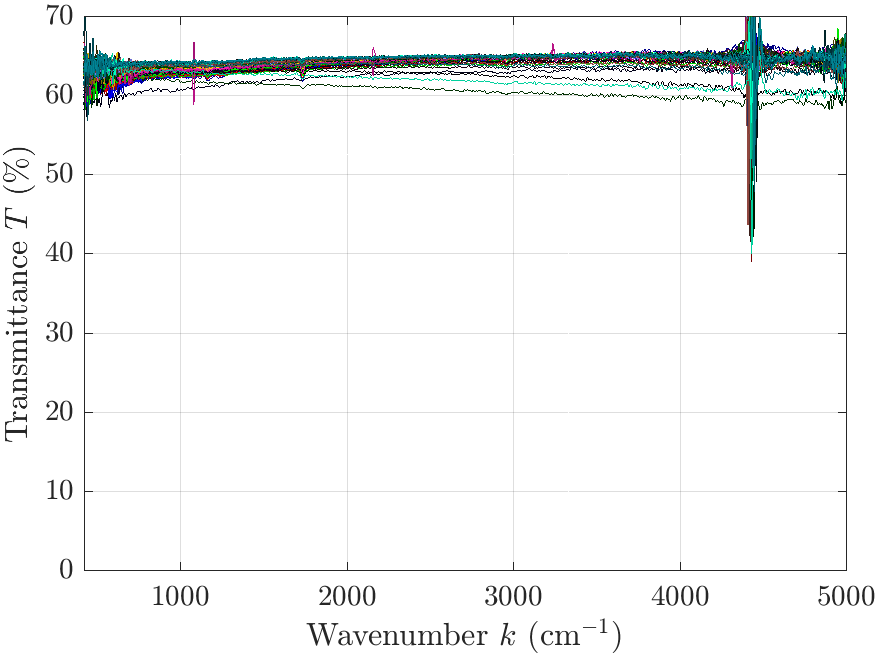
\includegraphics[width=0.7\linewidth]{subAa_121_ftir_spectra.png}
    \caption[\Ac{ftir} transmission spectra for the as-received substrate A.]{\Acf{ftir} transmission spectra recorded from a $11\times11$ grid on the as-received (111)B-oriented substrate A.}
    \label{fig:subAa_ftir_spectrum}
\end{figure}

The two factors that are mainly responsible for the reduction in \ac{ir} transmittance of \ac{czt} are the free carrier absorption and the scattering effect of precipitates \citep{yadava1994precipitation}. \citet{yujie2004infrared} used the transmittance at the wavenumber of $\SI{1000}{\centi\metre^{-1}}$ $T_{1000}$, the transmittance at the wavenumber of $\SI{5000}{\centi\metre^{-1}}$ $T_{5000}$, and the ratio of $T_{1000}$ to $T_{5000}$ to determine which of these two mechanisms that are the most significant. Their analysis gives a qualitatively determination of the density and size of \ce{Te} precipitates, the free carrier concentration, and the resistivity for \ac{czt} substrates.

Almost all the spectra from substrate A had a value of $T_{5000}$ between \SI{63}{\percent} and \SI{67}{\percent}, $T_{1000}$ between \SI{62}{\percent} and \SI{64}{\percent}, and a $T_{1000}/T_{5000}$ a little bit less than one. According to \citet{yujie2004infrared}, the \ac{czt} substrates with these characteristics are free of precipitates, have low free carrier concentration, and have resistivity that exceeds \SI{e6}{\ohm\centi\metre}.

\todo{Beskriv} Fig.~\ref{fig:subAa_ftir_map_500cm-1}

\begin{figure}[htbp]
    \centering
    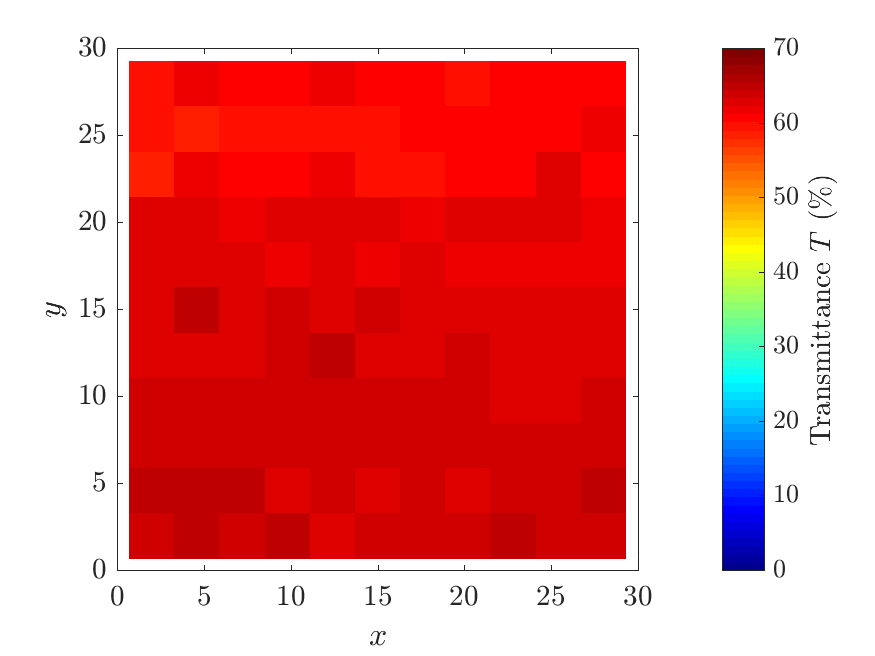
\includegraphics[width=0.7\linewidth]{subAa_121_ftir_transmission_at_k500cm-1.png}
    \caption[\Ac{ftir} transmission map for the as-received substrate A at $k=\SI{500}{\centi\metre^{-1}}$.]{\Acf{ftir} transmission map recorded from a $11\times11$ grid on the as-received (111)B-oriented substrate A at wavenumber $k=\SI{500}{\centi\metre^{-1}}$.}
    \label{fig:subAa_ftir_map_500cm-1}
\end{figure}

%%========================================
